\chapter{User Guide}

This appendix provides a walk-through of how to run and use the web application.

\section{Running the program}

The requirements before running the program are:

\begin{itemize}
	\item Python 2.7
	\item Django 1.10.5
	\item pandas 0.19.2
	\item django-graphos 0.3.23
	\item sklearn 0.0
	\item numpy 1.12.0
	\item scipy 0.18.1
	\item kmodes 0.7
\end{itemize}

Open terminal, go to the appropriate directory and enter the following:

\begin{lstlisting}
python manage.py runserver
\end{lstlisting}

Then open a browser and enter the following url:\par

\begin{lstlisting}
http://localhost:8000
\end{lstlisting}

The Home page should appear and you are ready to use the application.

\section{Home page}

Figure \ref{fig:homepage} shows an example of a home page. The navigation bar provides the main functions of the software. The page lists the groups which you have created, if you have not created a group yet it will be blank.

\begin{figure}[h]
\centering
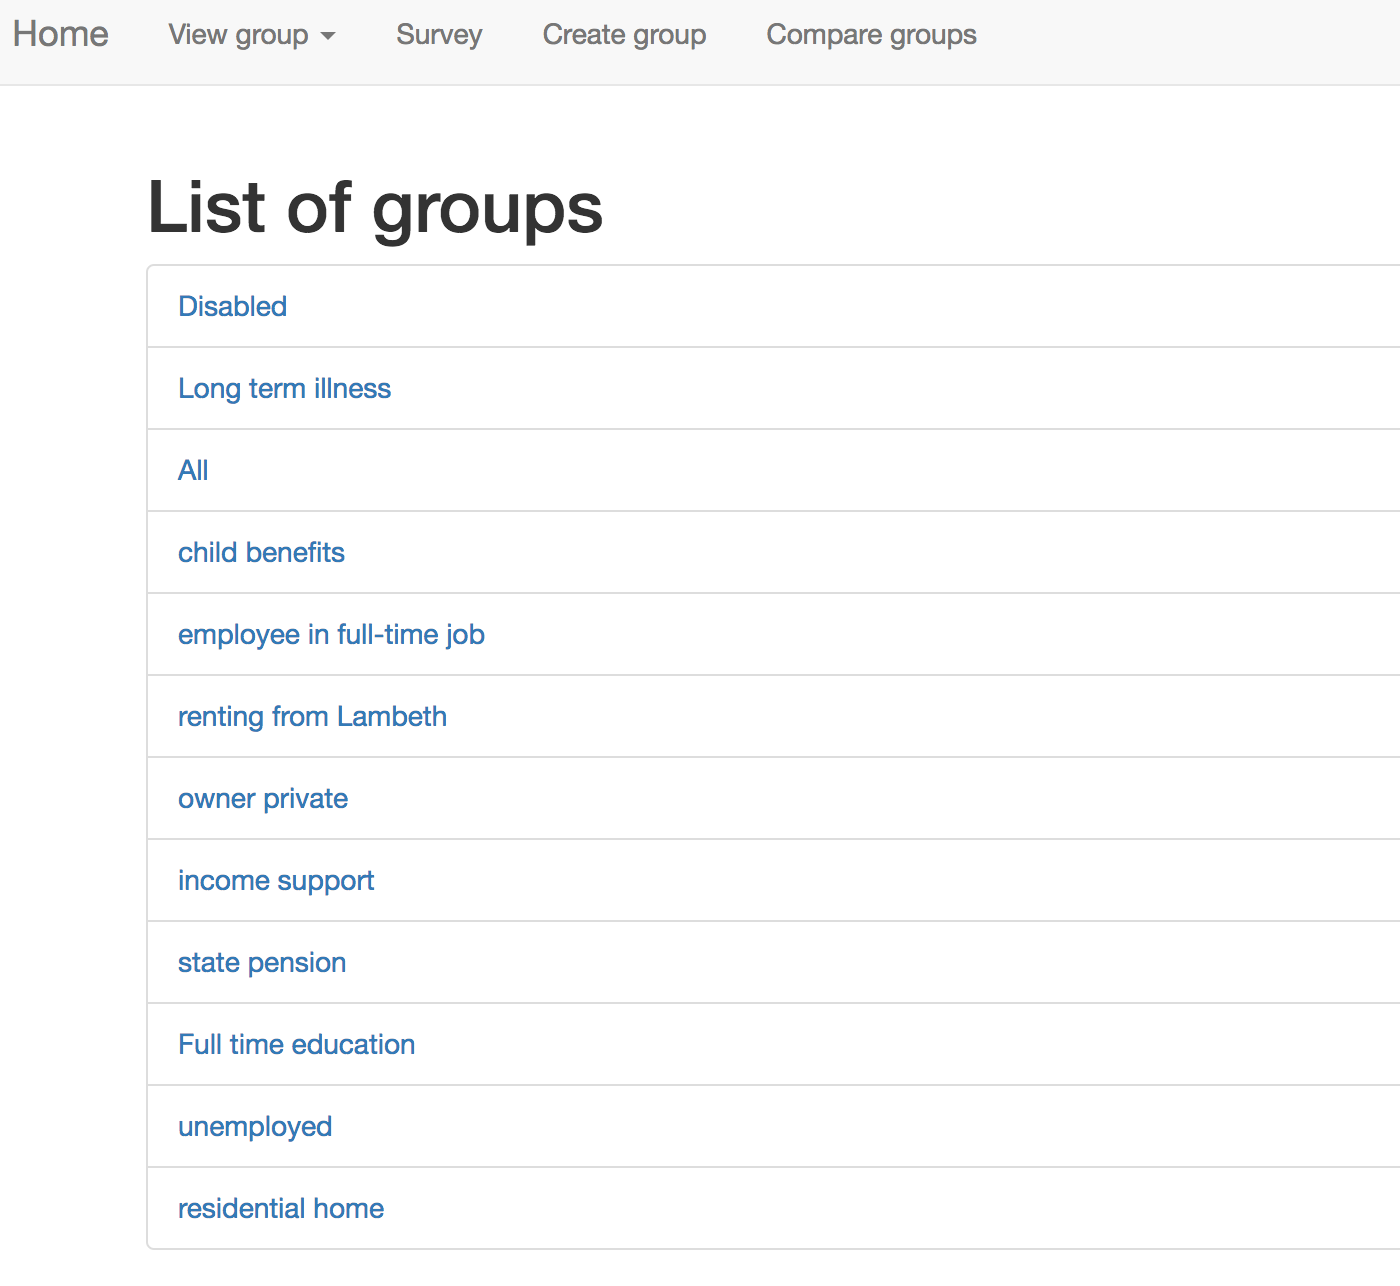
\includegraphics[scale=0.3]{homepage}
\caption{Screenshot of the homepage}
\label{fig:homepage}
\end{figure}

\section{Creating a group}

Begin by clicking on the ``Create group'' button on the navigation bar. The page in figure \ref{fig:creategrouppage} will appear. Enter the details for the group and then click ``Submit''. Ensure that the name of the group is not the same as other group names and each factor is filled out or else an error will appear.\par 

Select ``Any of the above'' if you do not wish to put anything for a factor.\par

\begin{figure}[h]
\centering
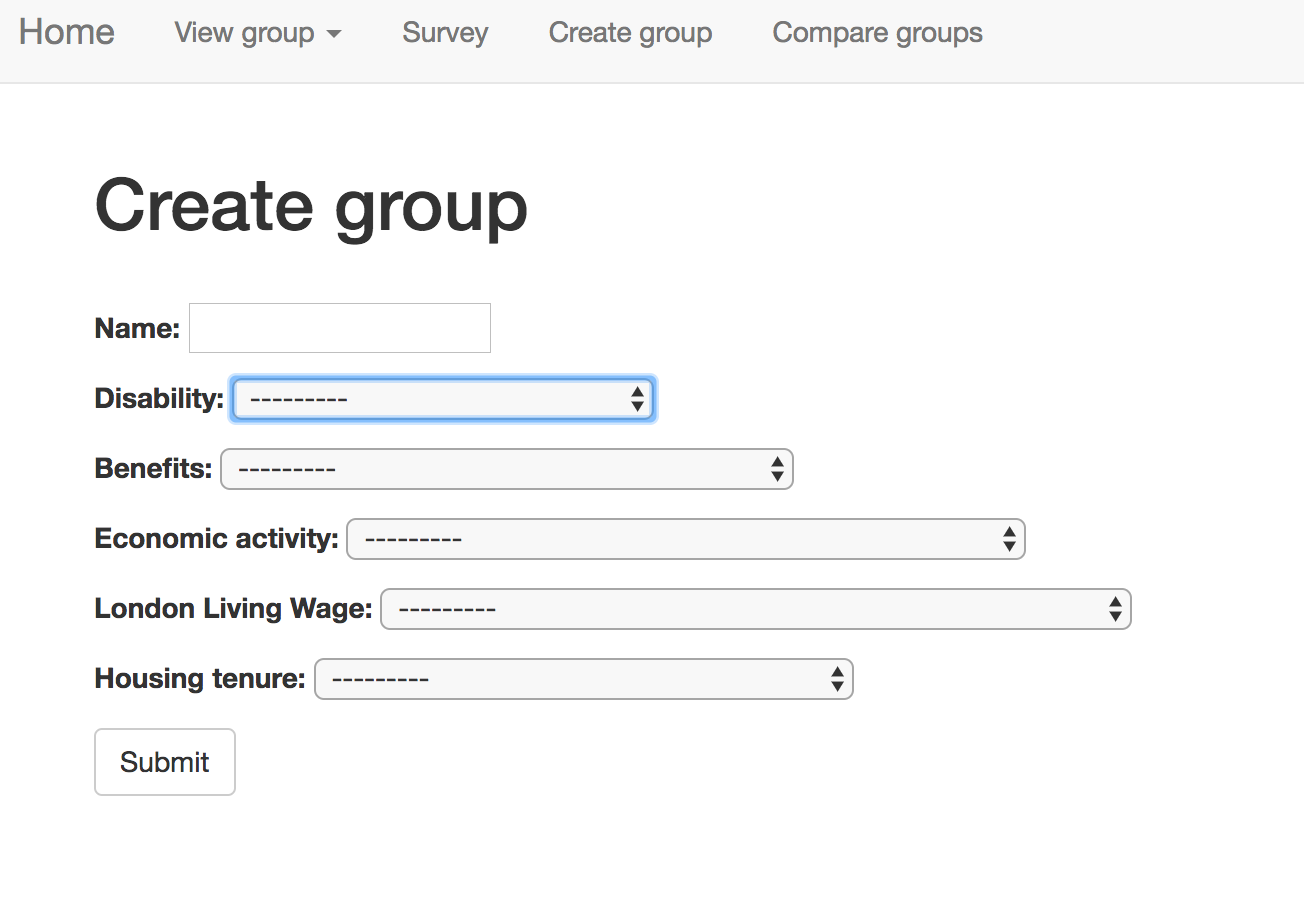
\includegraphics[scale=0.3]{creategrouppage}
\caption{Screenshot of the Create group page}
\label{fig:creategrouppage}
\end{figure}

View the group you have created by going to the home page or selecting it under ``View group'' in the navigation bar. The group detail page will appear (see section \ref{sec:groupdetailpage})

\section{Group pages} 

\subsection{Group detail page}
\label{sec:groupdetailpage}

The visualizations for the group could on this page. On the left side of the page shows the map divided into wards and Ward breakdown chart. The initial state of the map shows the population in each ward of the selected group. 

Hover over the map\textsc{\char13}s wards to view the name and value of the ward. The range above the map shows the meaning of the colors of the wards.

On the right side of the page are the charts of selected questions from Lambeth\textsc{\char13}s 2016 Residential Survey and the following buttons:

\begin{itemize}
	\item ``Refresh map'': Click to change the map to its default state i.e. showing the population of the current group.
	\item ``Compare clusters'': Click to compare data for each of the questions shown between data on the group\textsc{\char13}s clusters, the group and whole population.
	\item ``Stats'': Click to change the number of the group\textsc{\char13}s clusters and view the table of means for each question and cluster.
	\item ``Cluster n'': Click to view the visualization for this particular cluster number n.
	\item ``About group'': Click to view information about the factor setting, total population of the group, the source of the data and the number of clusters. There is also a delete button should you wish to delete this group.
	\item ``Edit group'': Click to edit the group\textsc{\char13}s name and factor settings.
	\item ``i'': Click to see instructions for this page.
\end{itemize}

\begin{figure}[h]
\centering
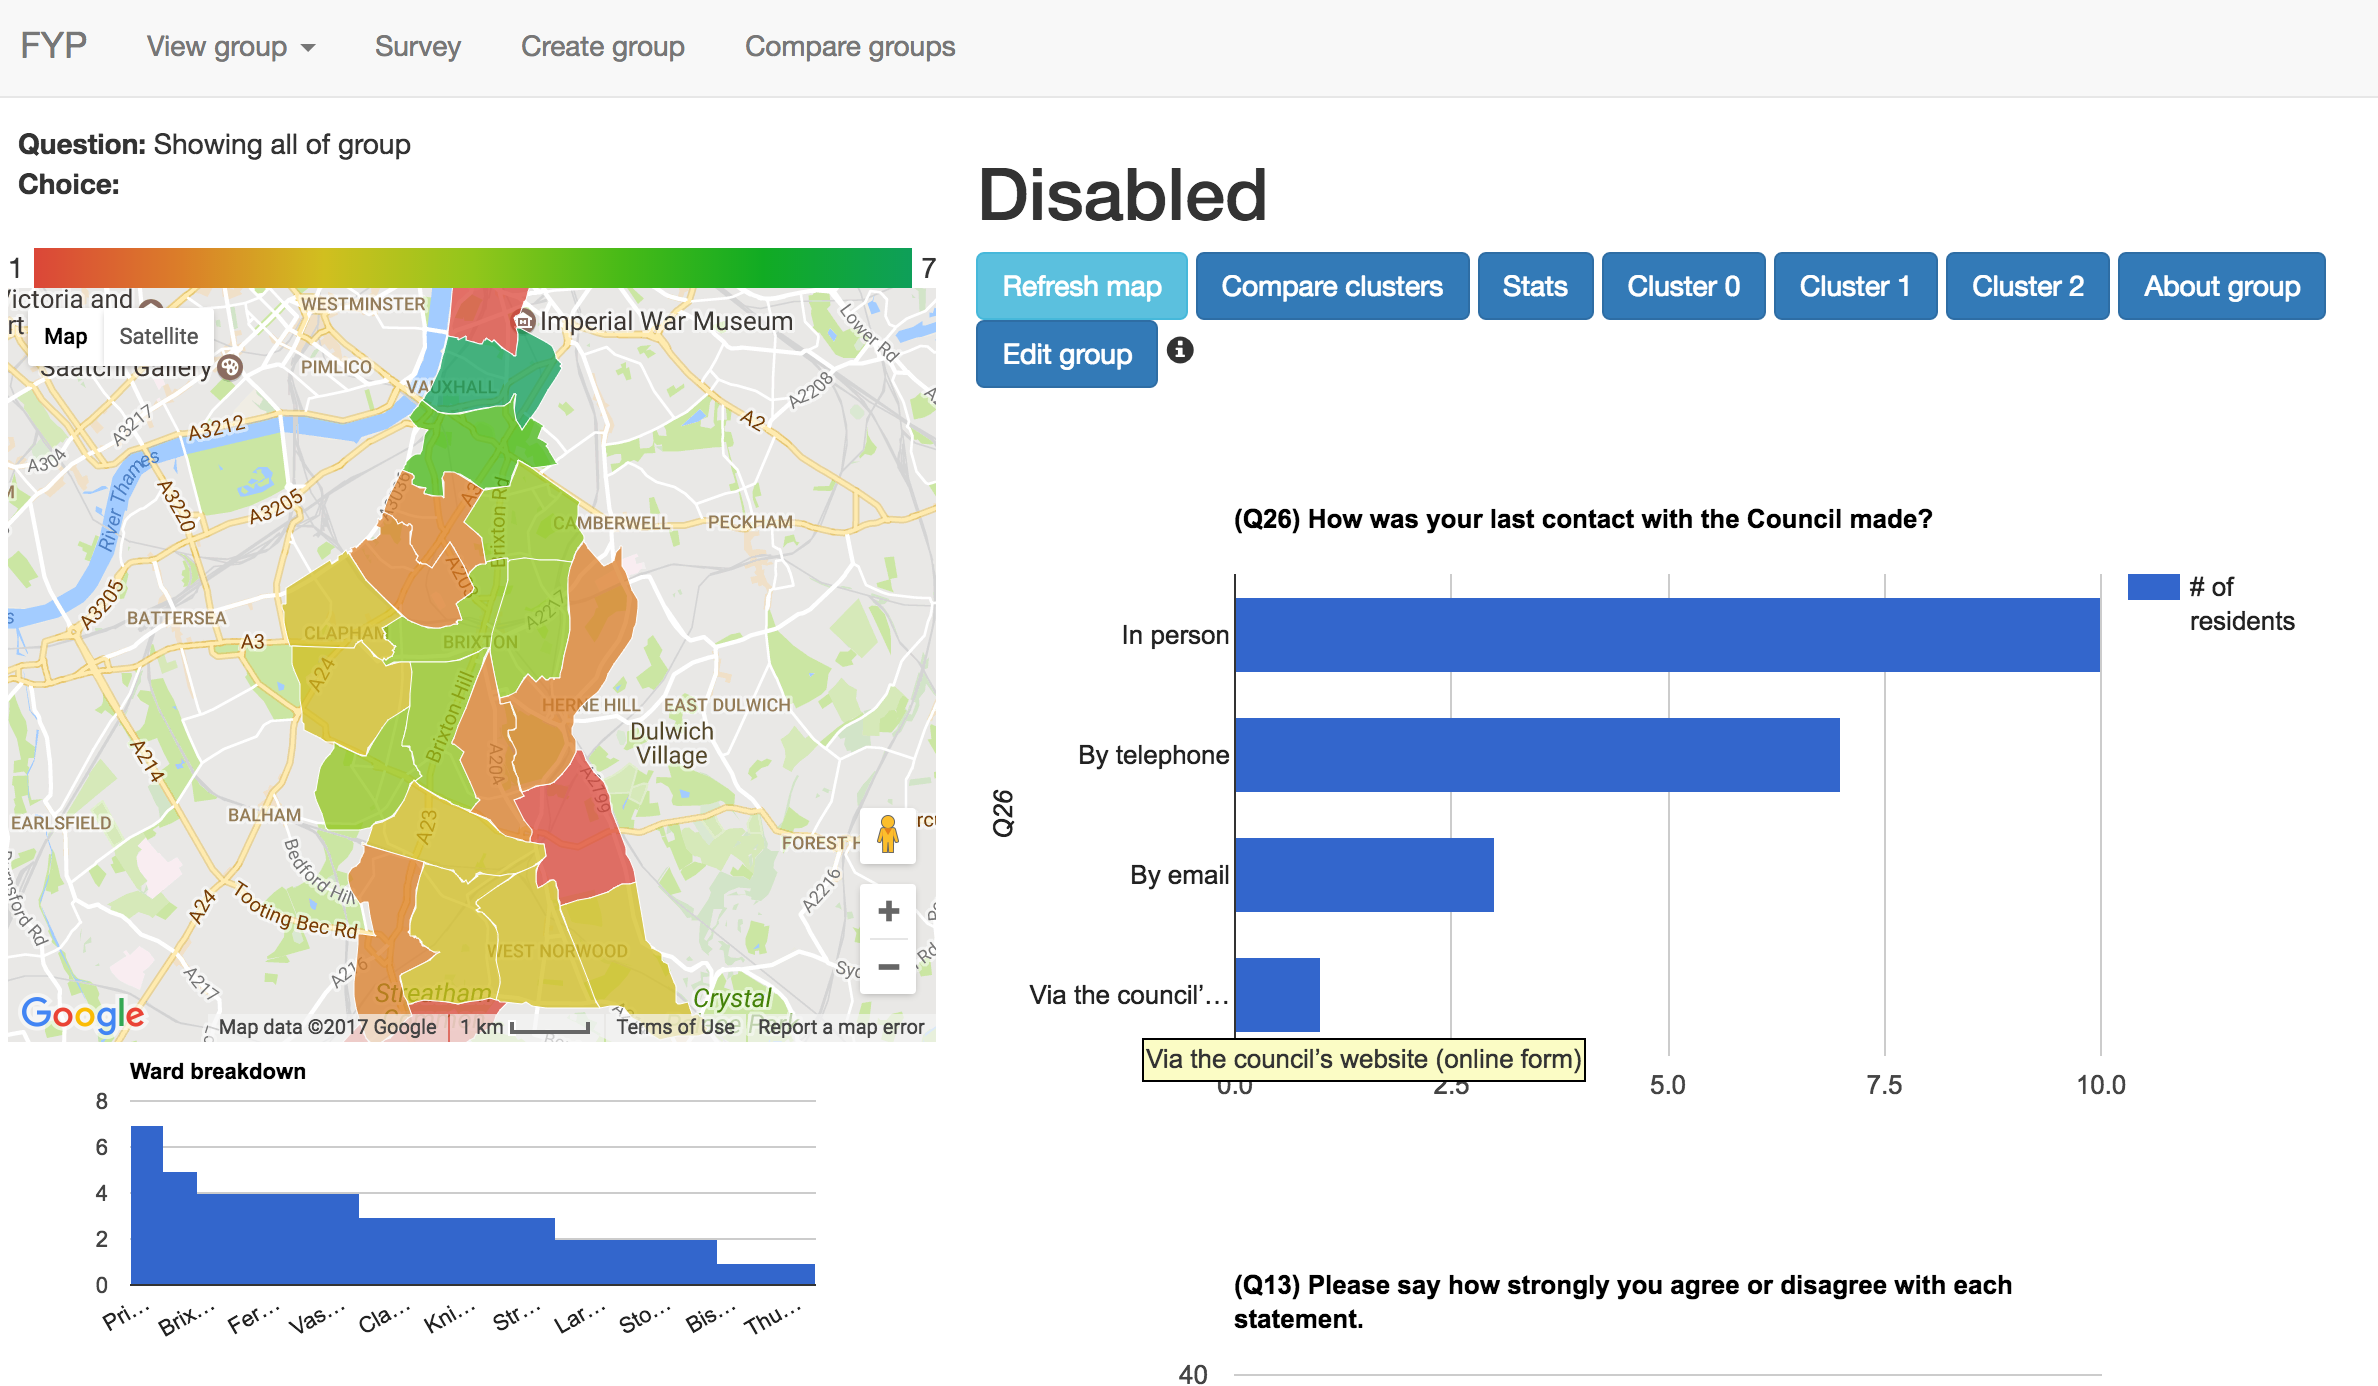
\includegraphics[scale=0.3]{figure3.png}
\caption{Screenshot of the Group detail page}
\label{fig:groupdetailpage}
\end{figure}

Some percentages are shown on the charts. Hover over the charts to view a tool tip of the percentage and original value of a variable. If in the legend, the whole text is not shown, hover over it and a tool tip of the whole text will appear.

\subsection{Compare clusters page}

This page seen in figure \ref{fig:compareclusterspage} allows the user to compare the results of each question between the whole population, the group and all of the group\textsc{\char13}s clusters. \par

The functionality of this page is similar to the Group detail page (see see \ref{sec:groupdetailpage})

\begin{figure}[h]
\centering
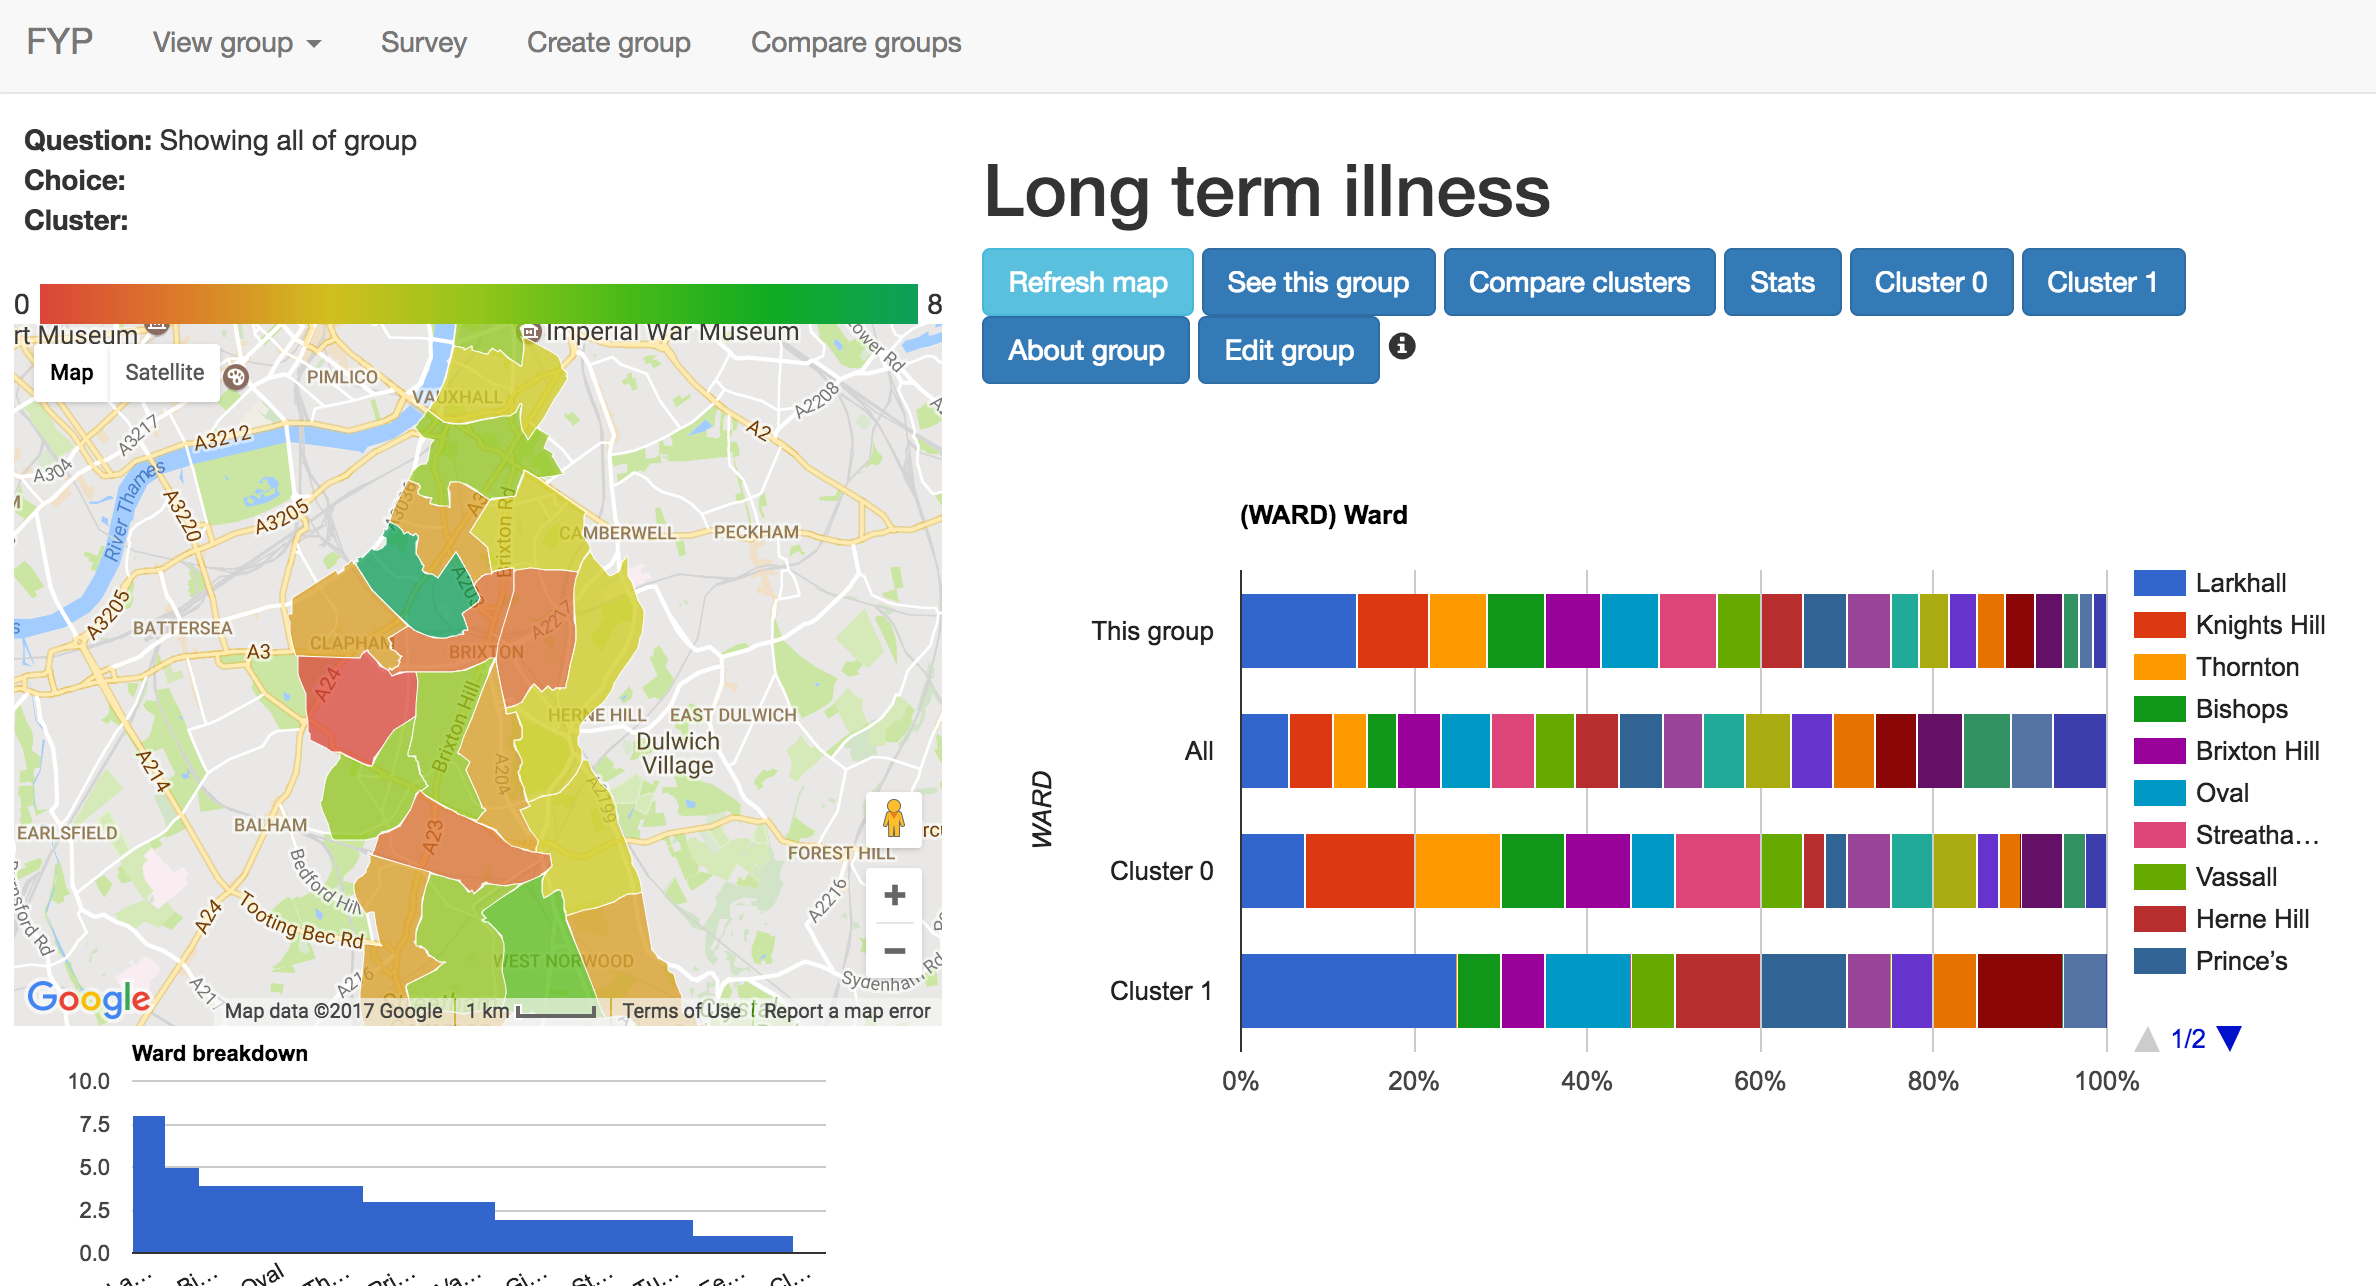
\includegraphics[scale=0.3]{comparisonpage}
\caption{Screenshot of the Compare clusters page}
\label{fig:compareclusterspage}
\end{figure}

\subsection{Stats page}

This page seen in figure \ref{fig:statspage} allows the user to change the number of clusters for this group. Clicking the up or down arrow will increase or decrease, respectively, the number of clusters. The system will not allow a number less than 1.\par

The Elbow chart aids the user in finding the optimal number of clusters using the elbow method. The biggest bend in the graph gives the optimal number of clusters. In figure\ref{fig:statspage} the number of clusters is 3. Choosing the bend tends to be subjective and may not always be clear which bend to choose. \par

\begin{figure}[h]
\centering
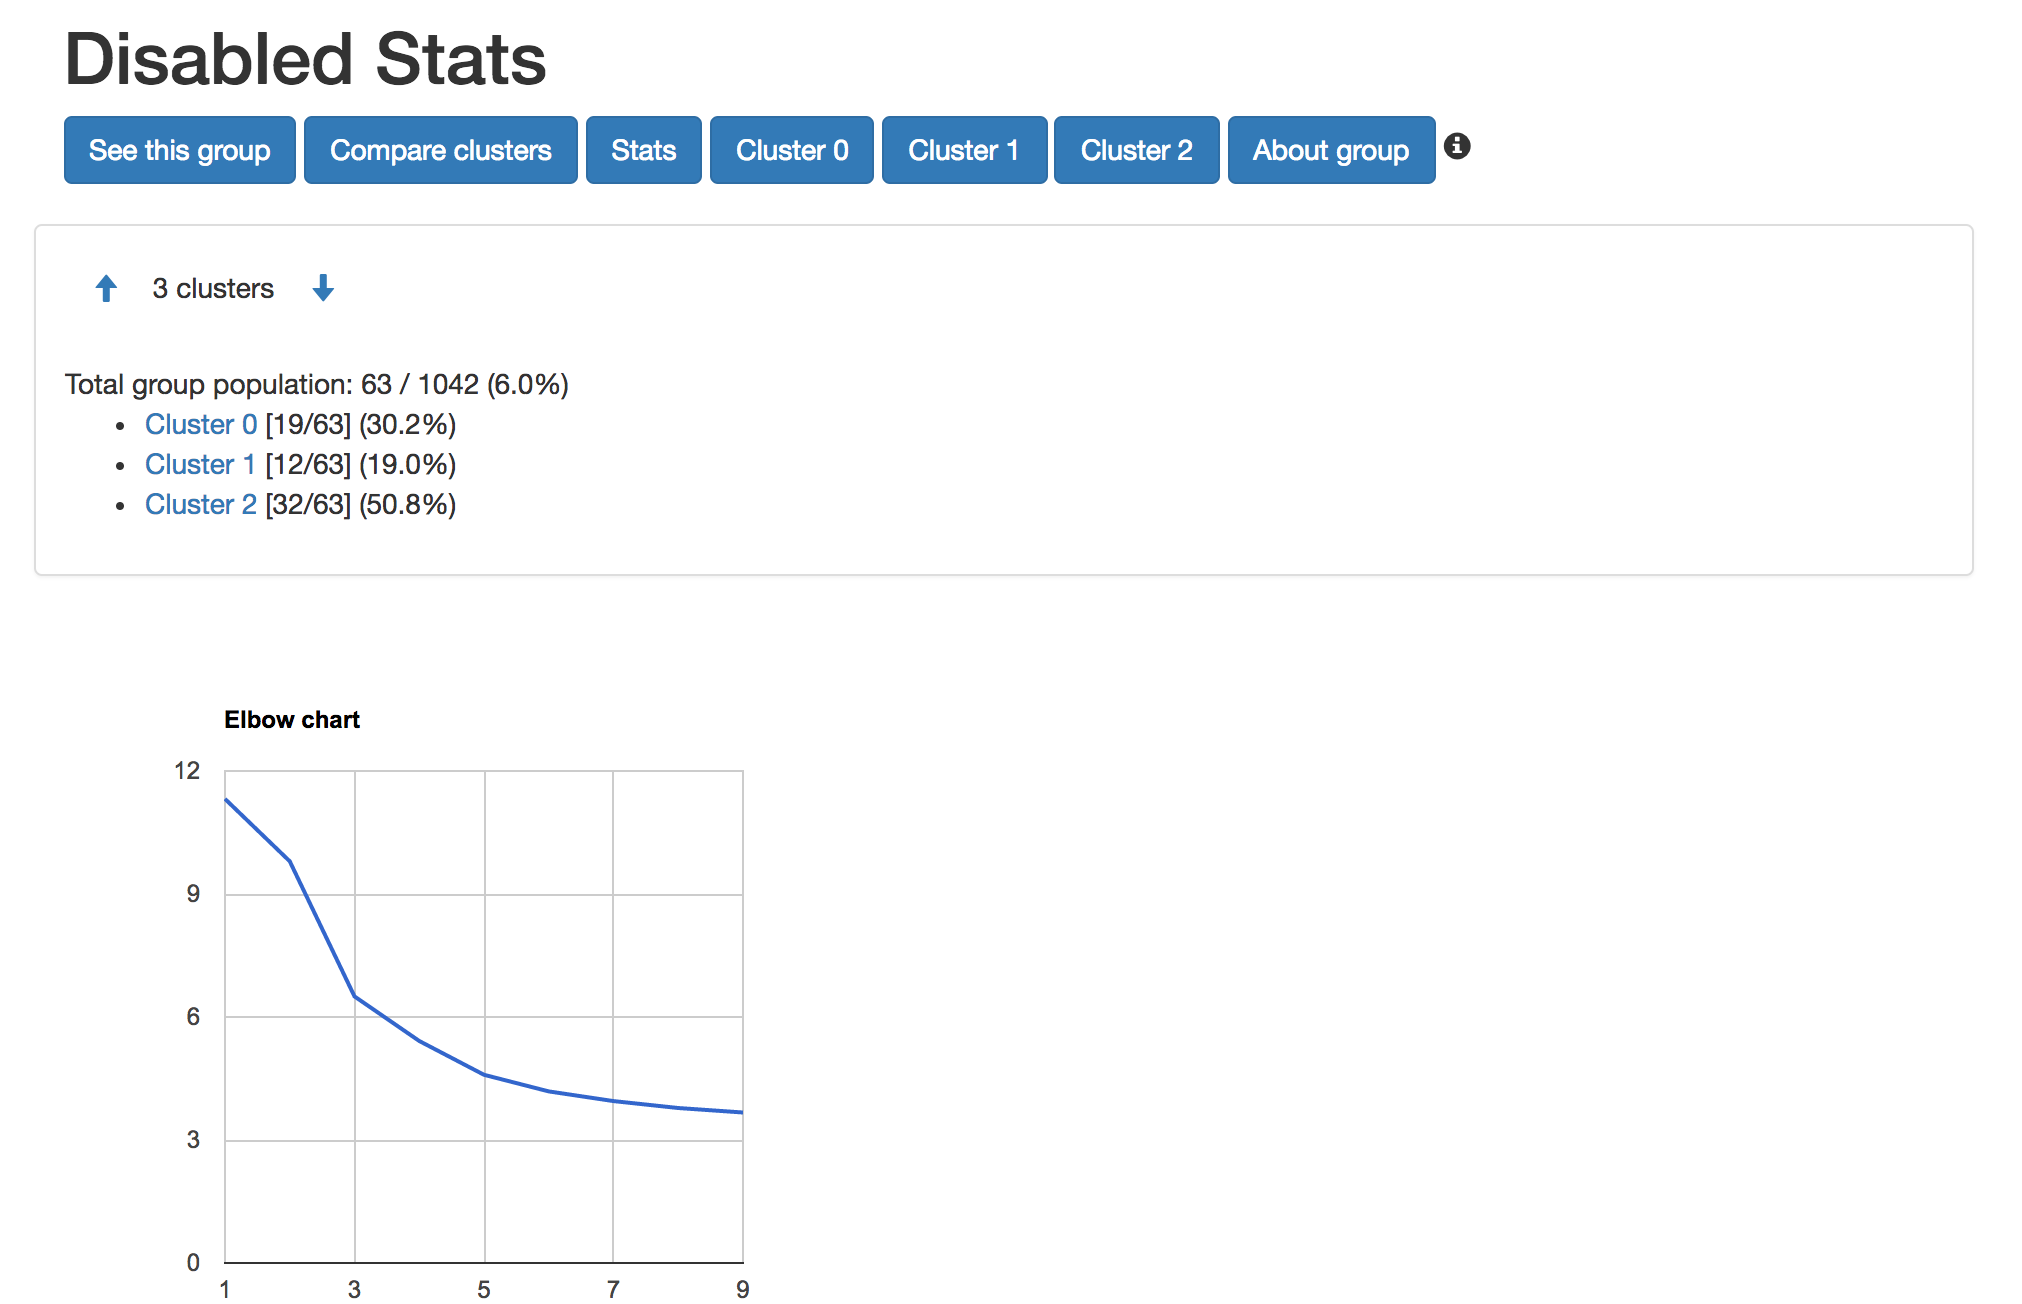
\includegraphics[scale=0.3]{statspage}
\caption{Screenshot of the Stats page}
\label{fig:statspage}
\end{figure}

Below the chart is the Table of mean values. The columns are the questions and the rows are the clusters. Therefore, values indicate the mean value for a question and cluster. This enables the user to identify differences between each cluster. For example see figure \ref{fig:tableofmeans}. Cluster 2 shows there may be a relation between Asian ethnicity (QETH), since the mean is 11 meaning Indian, and lower rating for belonging to the neighborhood (Q13\_R1), since the mean is around 2, compared to the other clusters, since their mean is around 1. 1 means they strongly agree that they belong to the neighborhood. 2 means they just agree. To see the distribution in more detail go to the Cluster detail page.

\begin{figure}[h]
\centering
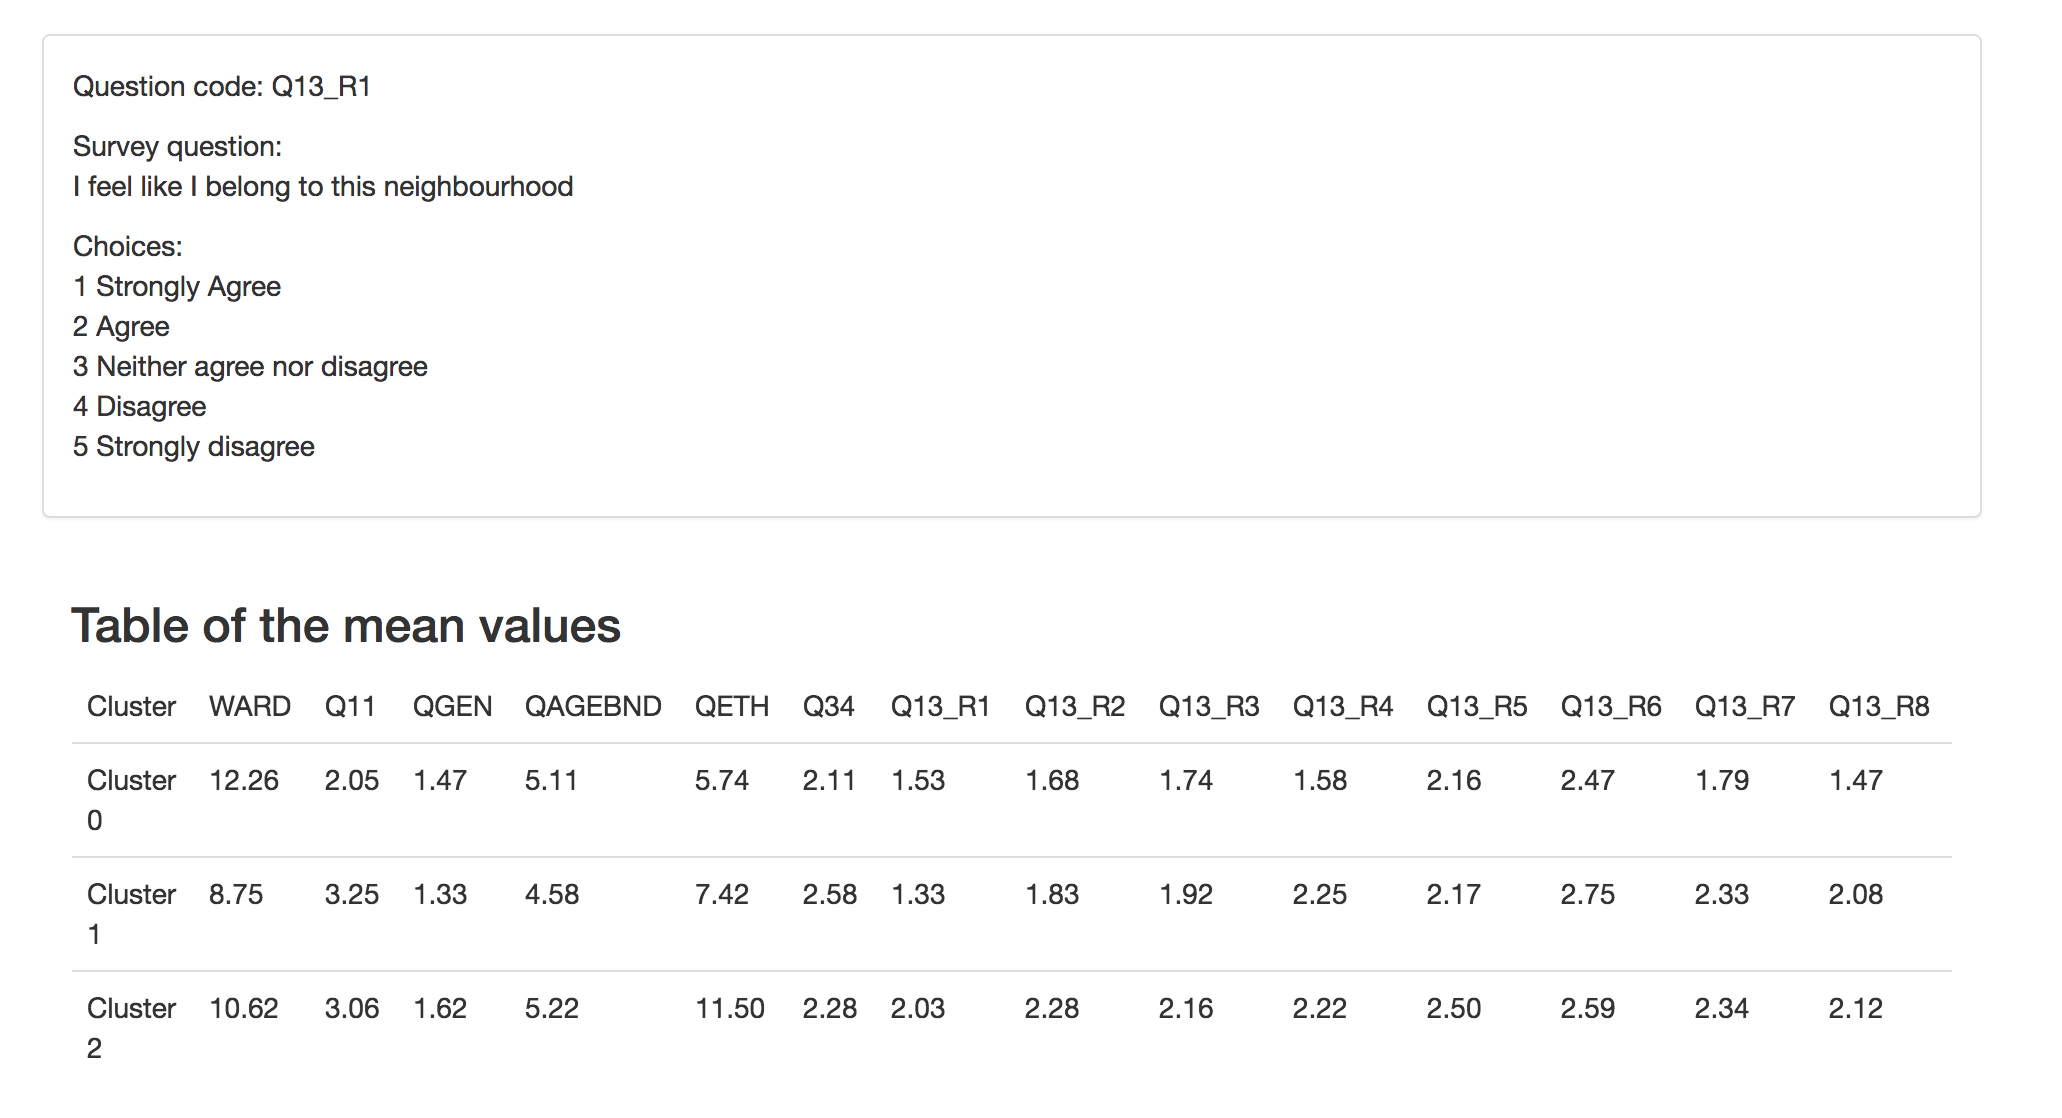
\includegraphics[scale=0.3]{tableofmeans}
\caption{Screenshot of the Table of means in the Stats page}
\label{fig:tableofmeans}
\end{figure}

Hovering over the question codes (e.g. Q11) will display the code translations above the table (see figure \ref{fig:tableofmeans}).

\subsection{Cluster detail page}

Clicking the ``Cluster n'' button, n is a number 	greater than 0, will show the visualizations for that cluster. The same functionalities described in section \ref{sec:groupdetailpage} are available on this page.

\section{Compare groups page}

Clicking the ``Compare groups'' button on the navigation bar will show the page shown in figure \ref{fig:groupcompare}.\par

\begin{figure}[h]
\centering
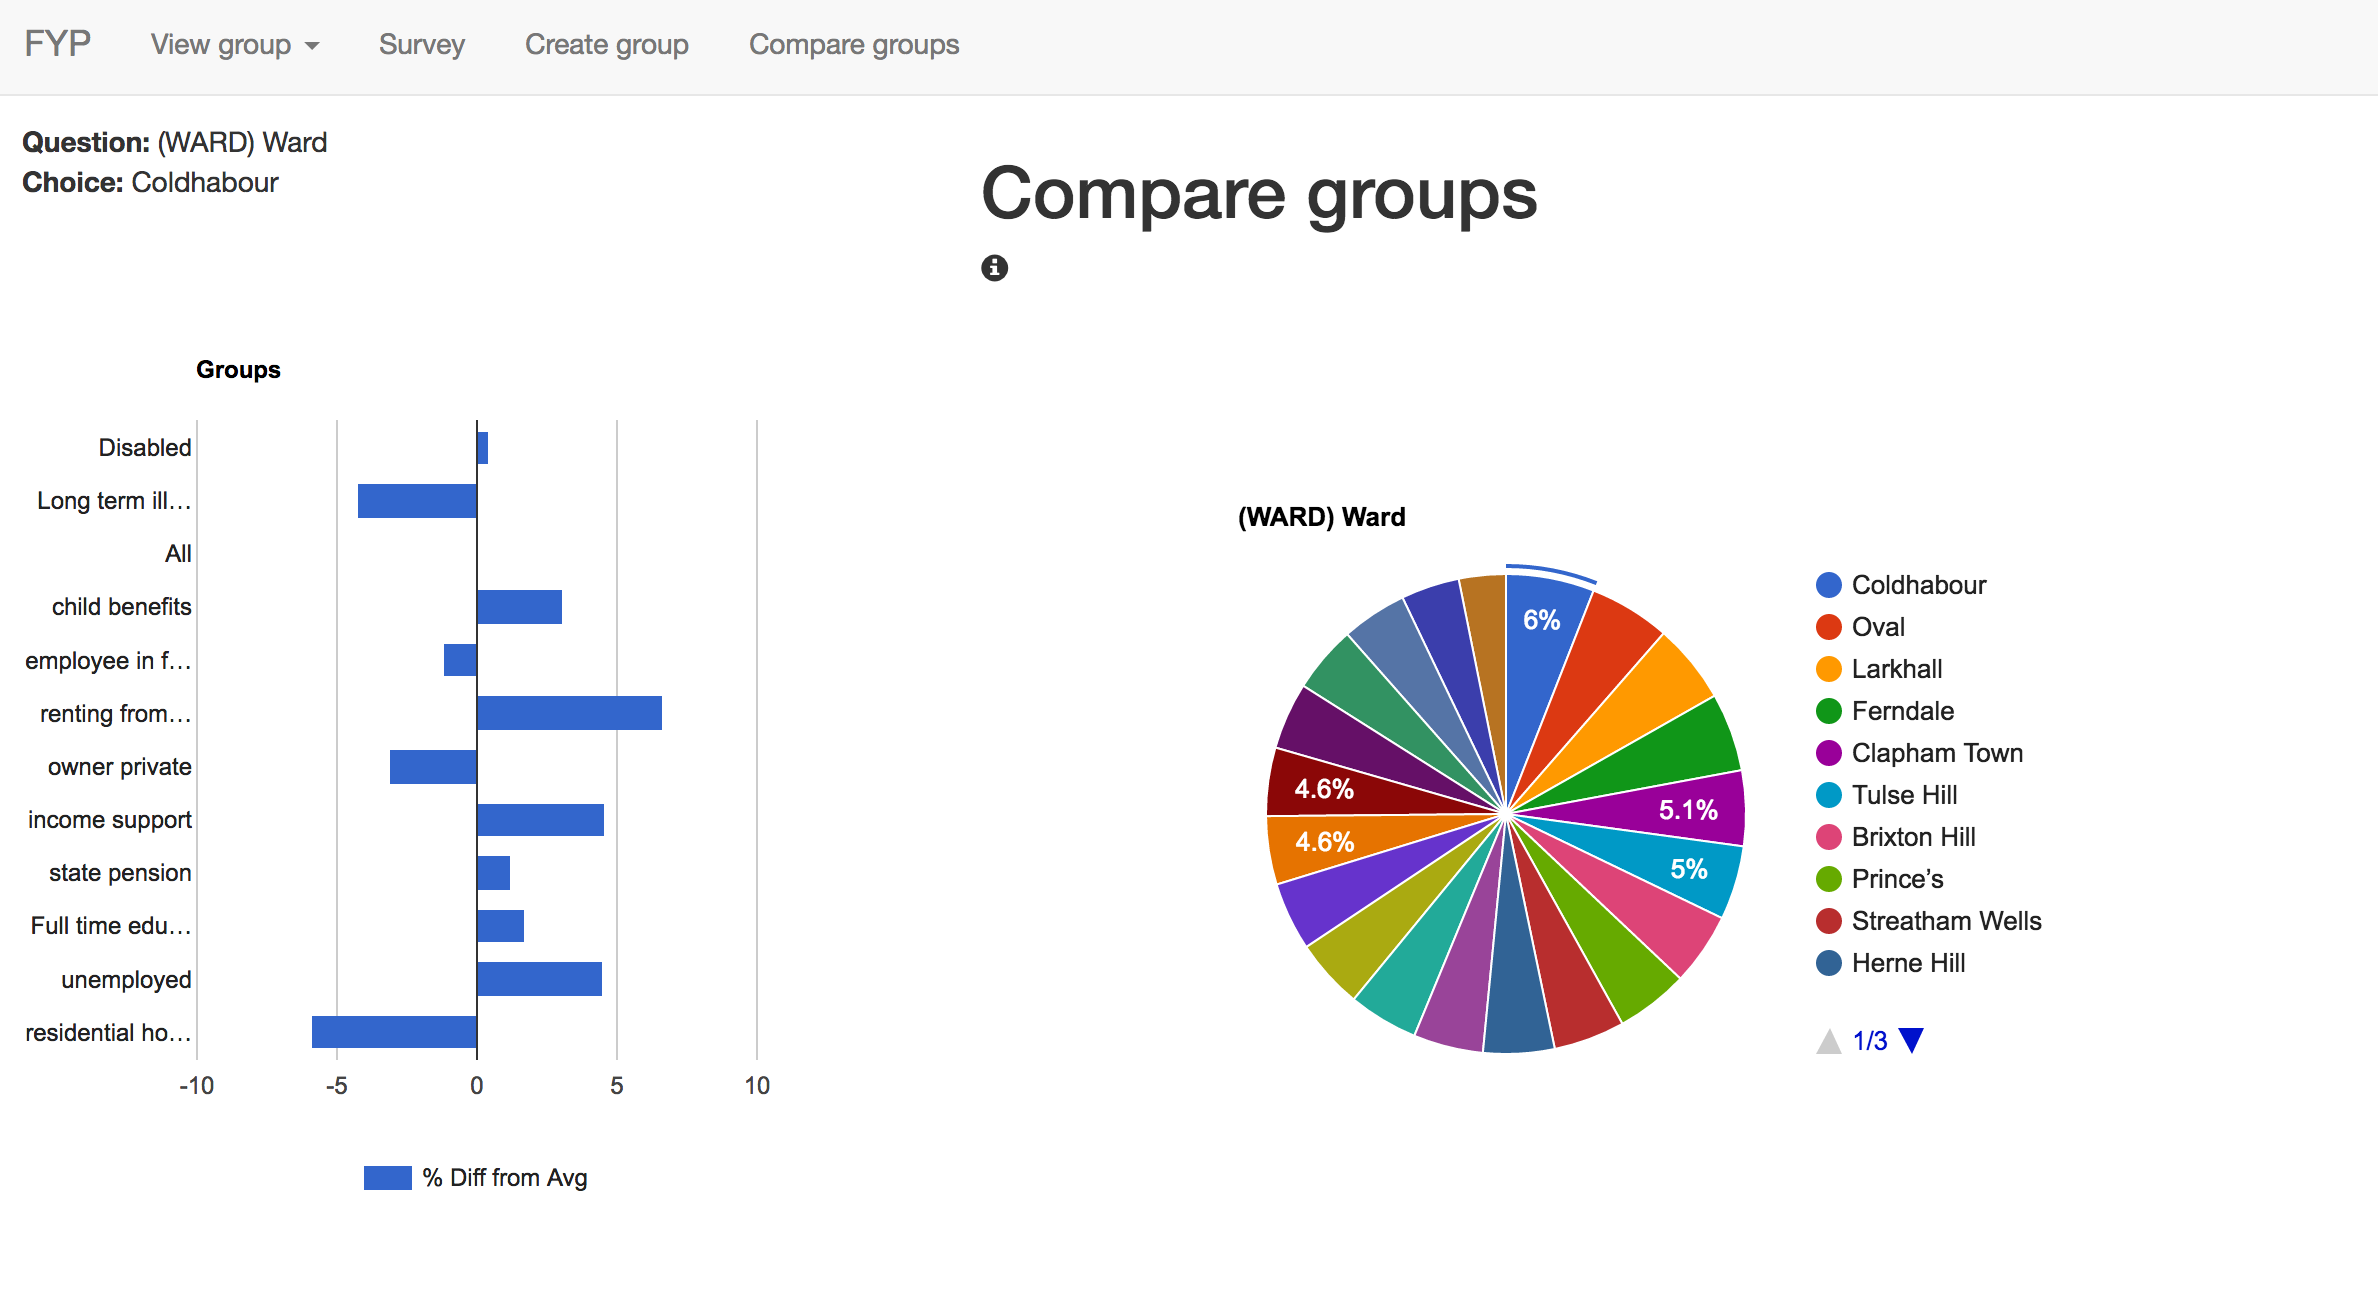
\includegraphics[scale=0.3]{groupcompare}
\caption{Screenshot of the Compare groups page}
\label{fig:groupcompare}
\end{figure}

On the left side of the page, the comparison of the groups could be seen as a chart. Groups on the right side of the line mean that they have a bigger proportion than the whole population which have the selected data variable.\par

On the right side of the page, the visualizations for the All group is displayed. Clicking the charts will display the selected data variable on the comparison chart on the left side of the page.\par

\section{Survey pages}

\subsection{Survey page}

Click on the ``Survey'' button on the navigation bar to go to this page (see figure \ref{fig:surveypage}). This page shows the links to the questions used in the system. Click a question and the Survey question page will appear (see section \ref{sec:questionpage}).

\begin{figure}[h]
\centering
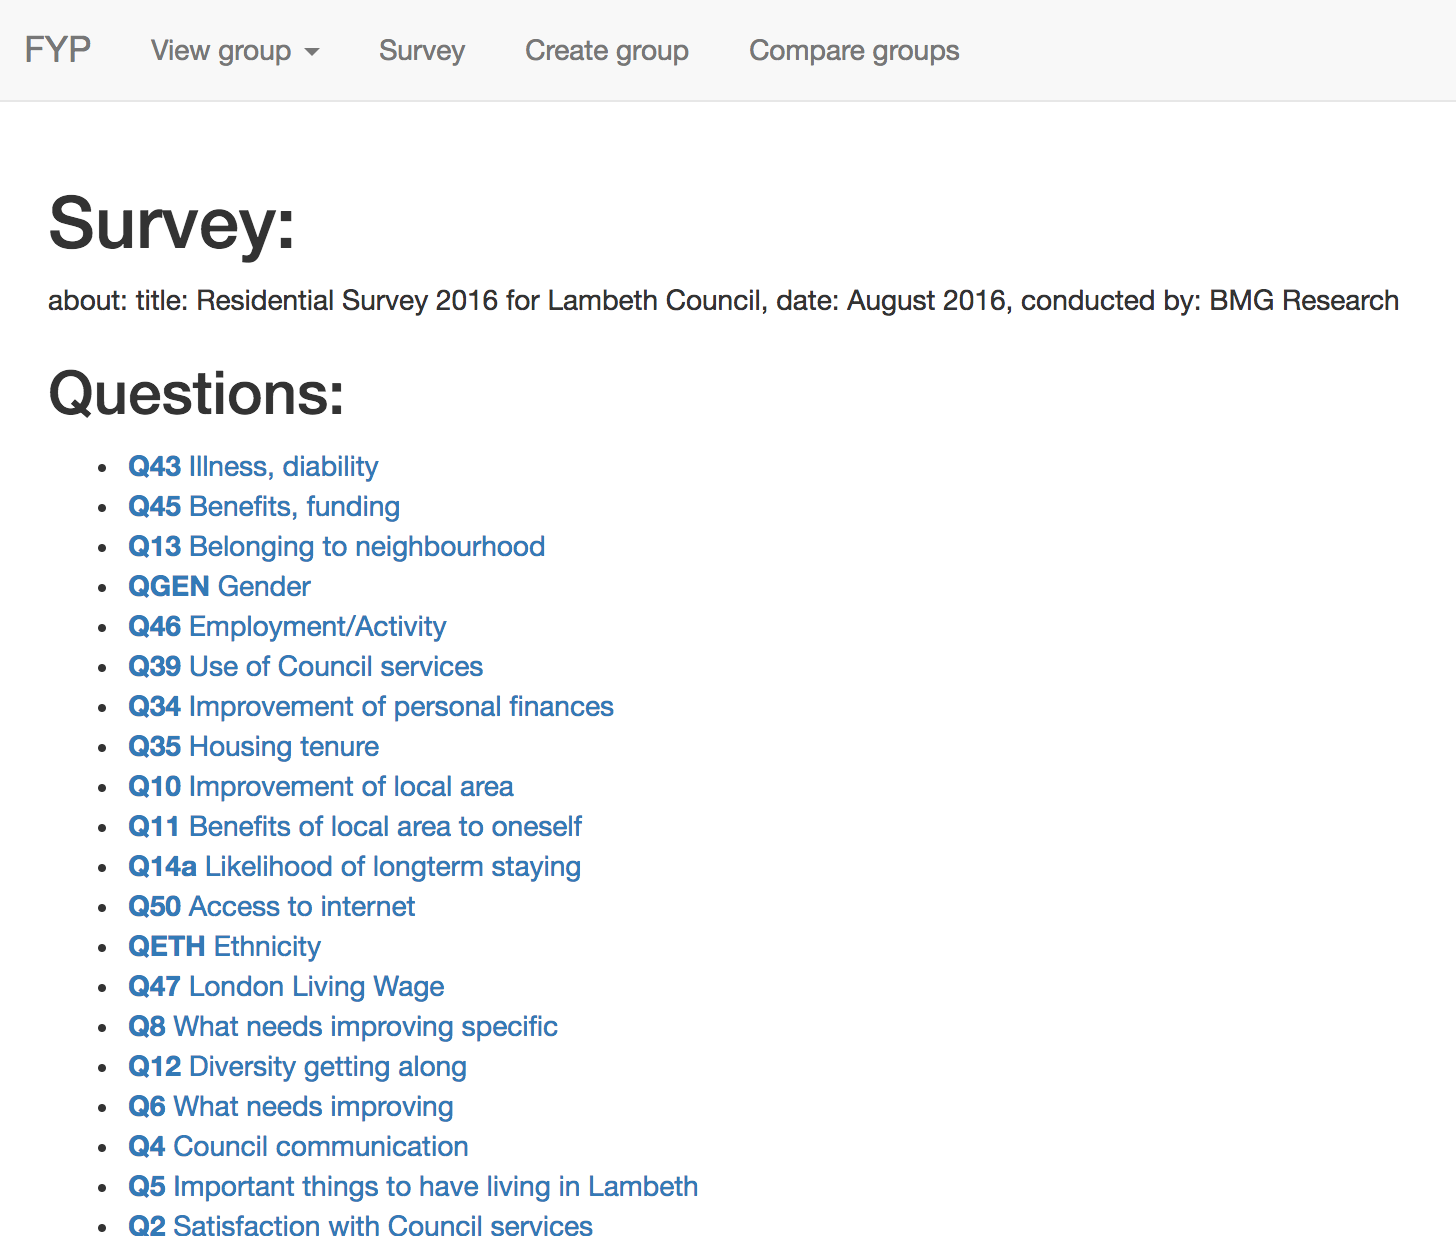
\includegraphics[scale=0.3]{surveypage}
\caption{Screenshot of the Survey page}
\label{fig:surveypage}
\end{figure}

\subsection{Survey question page} \label{sec:questionpage}

This page (see figure \ref{fig:surveyquestion}) visualizes the data of all groups on a single question. If the question is a multiple answer question, each subquestion is presented as a separate graph. This visualization is useful to see the differences in the proportions of each variable in each group.

\begin{figure}[h]
\centering
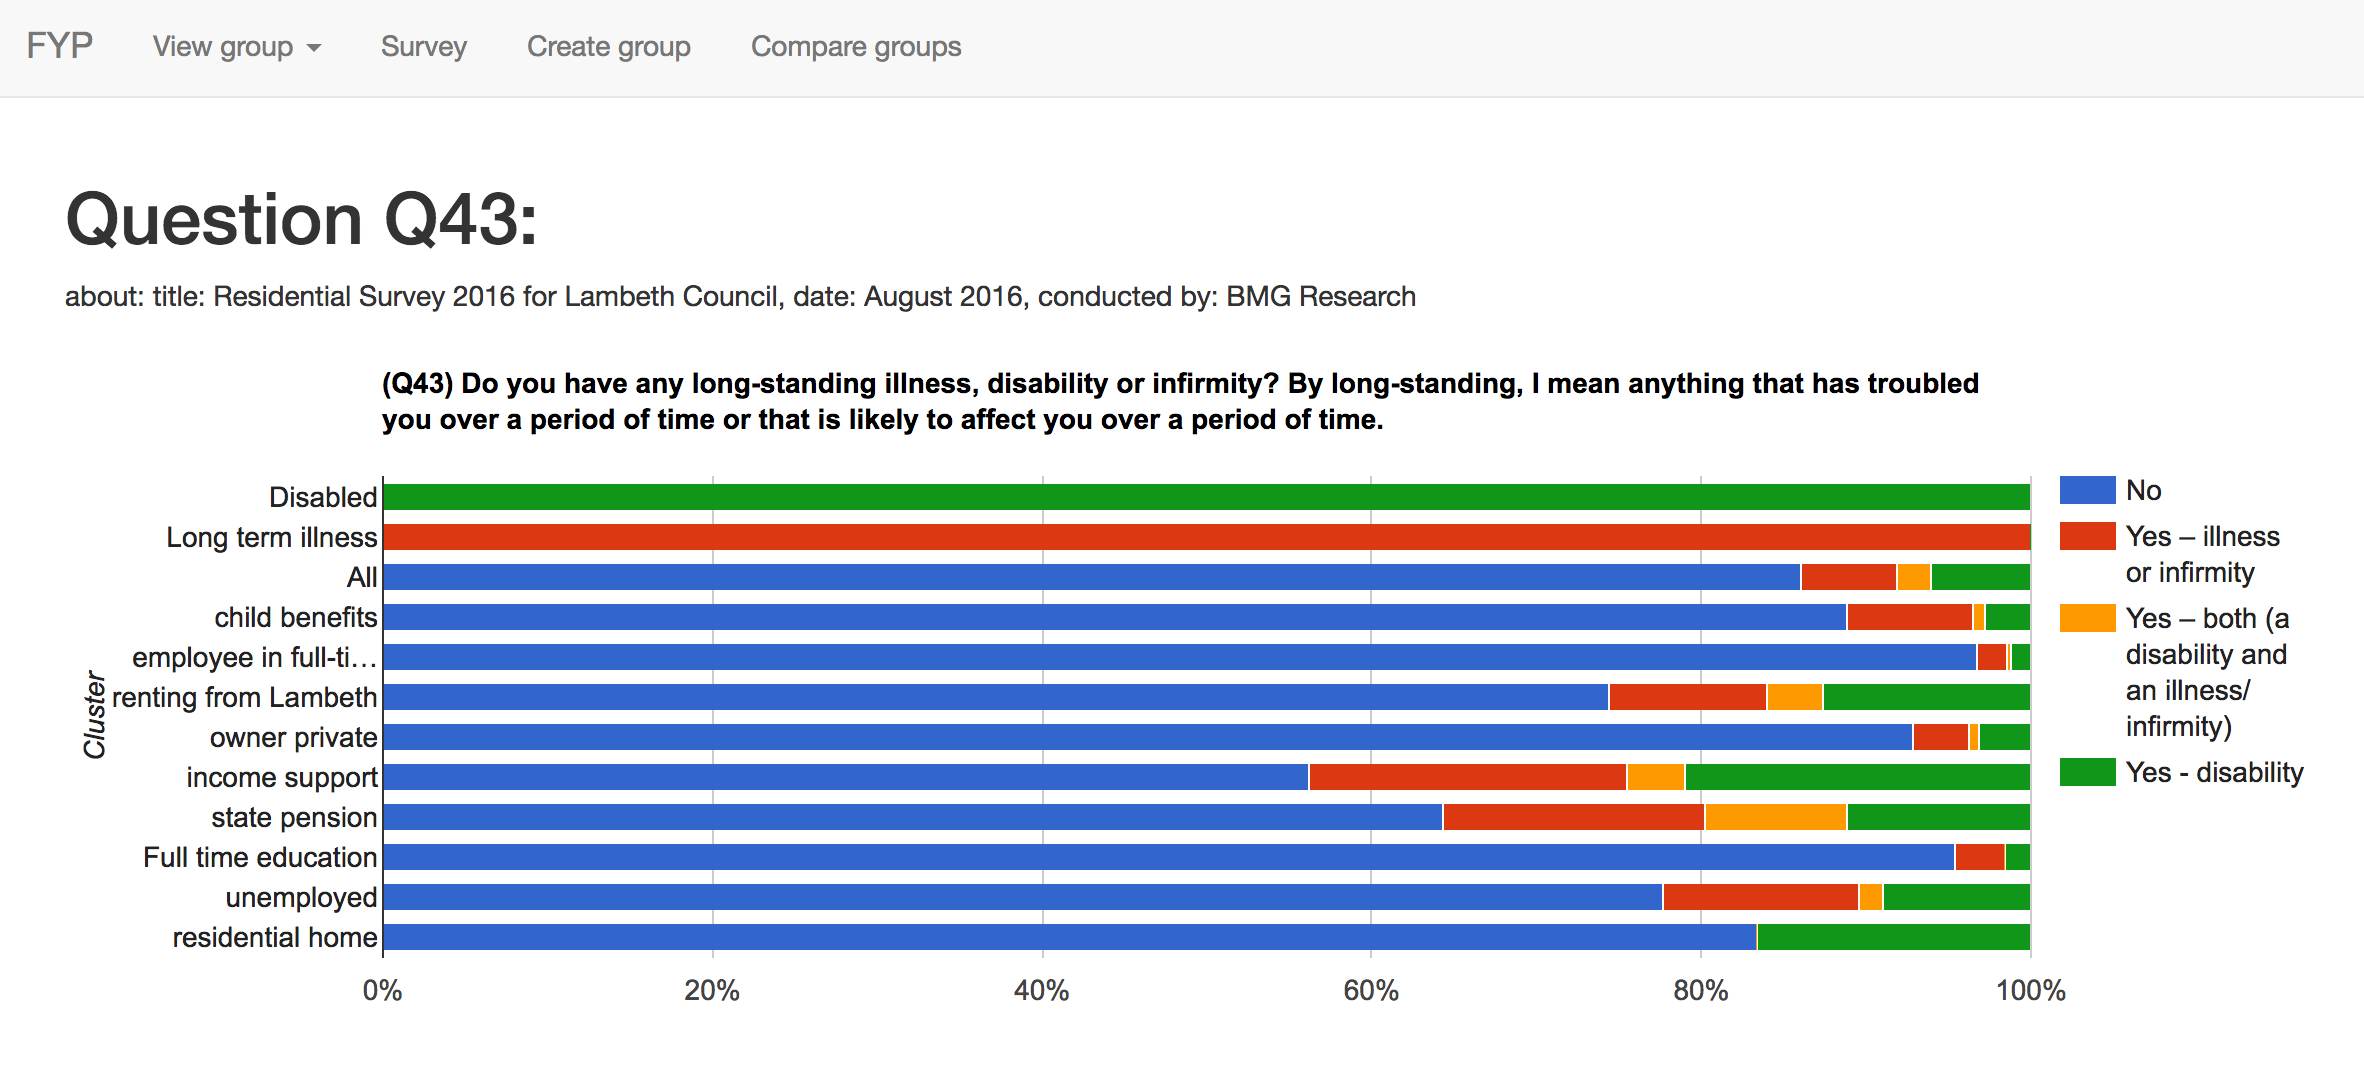
\includegraphics[scale=0.3]{surveyquestion}
\caption{Screenshot of the Survey question page}
\label{fig:surveyquestion}
\end{figure}